\documentclass{diploma}

\usepackage[table]{xcolor}
%\usepackage{pgfplots}
%\pgfplotsset{compat=1.16}

% Путь к рисункам
\graphicspath{{inc/Pictures}}
\student{Садаков Александр Александрович}
\group{М8О-207М-23}
\theme{Численное моделирование течения струй газа с неравновесным химическим процессом}

\supervisor{Демидова Ольга Львовна}
\firstConsultant{---}
\secondConsultant{---}
\reviewer{---}

\faculty{№ 8 <<Компьютерные науки и прикладная математика>>}
\department{806}
\speciality{01.03.02 <<Прикладная математика и информатика>>}
\profile{Информатика}

\departmentFullName{№ 806}
\headOfDepartment{Крылов Сергей Сергеевич}

% Дата. Оставляем пустое место для дня
\date{\uline{\hspace{24pt}} мая \the\year\ года}

\newacronym{du}{ДУ}{дифференциальное уравнение}
\newacronym{odu}{ОДУ}{обыкновенное дифференциальное уравнение}
\newacronym{sdu}{СДУ}{система дифференциальных уравнений}
\newacronym{snu}{СНУ}{система нелинейных уравнений}
%\newacronym{sau}{САУ}{система алгебраических уравнений}
%\newacronym{slau}{СЛАУ}{система линейных алгебраических уравнений}
\newacronym{rho}{$\rho$}{плотность, $\dfrac{\text{кг}}{\text{м}^3}$}
\newacronym{t}{$t$}{время, $\text{с}$}
\newacronym{P}{$P$}{давление, $\text{Па}$}
\newacronym{T}{$T$}{температура, $\text{К}$}
\newacronym{V}{$V$}{объём, $\text{м}^3$}
\newacronym{R}{$R$}{универсальная газовая постоянная, $\dfrac{\text{Дж}}{\text{К} \cdot \text{моль}}$}
\newacronym{U}{$U$}{внутренняя энергия, $\dfrac{\text{Дж}}{\text{кг}}$}
\newacronym{N}{$N$}{число компонентов в смеси}
\newacronym{G}{$G$}{потенциал Гиббса, $\dfrac{\text{Дж}}{\text{кг}}$}
\newacronym{gamma}{$\gamma_i$}{мольно-массовая концентрация i-го компонента, $\dfrac{\text{моль}}{\text{кг}}$}
\newacronym{mu}{$\mu_i$}{химический потенциал i-го компонента, $\dfrac{\text{Дж}}{\text{моль}}$}
\newacronym{Nr}{$N_R$}{число реакций}
\newacronym{Wi}{$W_i$}{скорость образования i-го компонента, $\dfrac{\text{моль}}{\text{м}^3 \cdot \text{с}}$}
\newacronym{nu}{$\nu^{(r)}$}{стехиометрические коэффициенты}
\newacronym{Wr}{$W^{(r)}$}{скорости r-ой химической реакции, $\dfrac{\text{моль}}{\text{м}^3 \cdot \text{с}}$}
\newacronym{q}{$q^{(r)}$}{молекулярность r-ой элементарной реакции}
%ещё из химии посмотреть
%все буквы из формул
\newglossaryentry{id1}{ % Нужны разные id, можно ставить просто последовательно
    name={Жёсткая система},
    description={ОДУ, численное решение которого явными методами является неудовлетворительным из-за резкого увеличения
    числа вычислений или из-за резкого возрастания погрешности при недостаточно малом шаге} 
}
\newglossaryentry{id2}{
    name={Методы Рунге-Кутты},
    description={большой класс численных методов решения задачи Коши для обыкновенных дифференциальных уравнений и их систем} 
}
\newglossaryentry{id3}{
    name={Условие химического равновесия},
    description={равенство полных химических потенциалов исходных веществ и продуктов} 
}
\newglossaryentry{id4}{
    name={Химическая кинетика},
    description={раздел физической химии, изучающий закономерности протекания химических реакций во времени, зависимости этих
    закономерностей от внешних условий, а также механизмы химических превращений} 
}
\newglossaryentry{id5}{
    name={Критерий Рейнольдса},
    description={отношение инерционных сил к вязким, определяющее этапы перехода от ламинарных течений к турбулентным} 
}
\newglossaryentry{id6}{
    name={Турбулентность},
    description={сложное, неупорядоченное во времени и пространстве поведение диссипативной среды (или поля), детали которого не могут быть воспроизведены на больших интервалах времени при сколь угодно точном задании начальных и граничных условий} 
}
\newglossaryentry{id7}{
    name={Ламинарный поток},
    description={упорядоченное течение жидкости или газа, при котором жидкость или газ перемещается как бы слоями, параллельными направлению течения} 
}
\newglossaryentry{id8}{
    name={Турбулентная вязкость},
    description={мера сопротивления течению, вызванного турбулентными флуктуациями} 
}
\newglossaryentry{id9}{
    name={Число Прандтля},
    description={характеристика влияния свойств жидкости на интенсивность теплообмена, являющаяся критерием подобия температурного и скоростного полей, а также описывает свойства теплоносителя} 
}
\newglossaryentry{id10}{
    name={Число Шмидта},
    description={отношение коэффициентов кинематической вязкости и диффузии, описывающее относительную роль молекулярных процессов переноса количества движения и переноса массы примеси диффузией} 
}
\newglossaryentry{id11}{
    name={Число Льюиса},
    description={соотношение между интенсивностями переноса массы компонента диффузией и переноса теплоты теплопроводностью, пользующееся для характеристики потоков жидкости, в которых одновременно происходит тепломассообмен} 
}
\newglossaryentry{id12}{
    name={Неравновесный химический процесс},
    description={реакция, скорость которой определяется кинетикой, а не термодинамическим равновесием} 
}
\newglossaryentry{id13}{
    name={Скорость химической реакции},
    description={изменение концентрации реагентов или продуктов во времени} 
}
\newglossaryentry{id14}{
    name={Сетка (расчётная область)},
    description={дискретное представление пространства, на котором решаются уравнения} 
}
\newglossaryentry{id15}{
    name={Ламинарное горение},
    description={режим горения без турбулентных пульсаций} 
}
\newglossaryentry{id16}{
    name={Турбулентное горение},
    description={горение, осложнённое турбулентным перемешиванием} 
}
\newglossaryentry{id17}{
    name={Параболизированные уравнения Навье-Стокса},
    description={упрощённая система уравнений, в которой пренебрегают обратными течениями, сохраняя только доминирующее направление потока} 
}
\newglossaryentry{id18}{
    name={Струйное течение},
    description={течение газа, истекающего из сопла или отверстия в окружающую среду} 
}
\newglossaryentry{id19}{
    name={Пограничный слой},
    description={тонкая область у поверхности, где вязкие эффекты существенны} 
}
\newglossaryentry{id20}{
    name={Верификация},
    description={проверка корректности реализации численного метода} 
}
\newglossaryentry{id21}{
    name={Валидация},
    description={сравнение результатов моделирования с экспериментальными данными} 
}


\addbibresource{main.bib}

% Иллюстрации всегда по центру
\makeatletter
\g@addto@macro\@floatboxreset\centering
\makeatother

\begin{document}
    \maketitle

    %\includepdf[pages=-]{extra/task} % Задание
    \setcounter{page}{2} % Устанавливает счётчик страниц

    % O текст про жёсткость (ссылки)
% O устойчивость (а-, л-устойчивость, критерии устойчивости)
% O литература (30-40)
% V полунеявные методы в отдельный пункт
% O списки и переносы на новые страницы
% V уменьшить шрифт букв на картинках
% V поменять пунк про пользовательский интерфейс и парсер (вывод для парсера)
% V названия для задач
% O убрать температуру и давление из систем (перенести их на строчку повыше)
% V бомба в отдельный заголовок
% V апробация

\abstract % Структурный элемент: РЕФЕРАТ
%количество источников

\keywords{ЧИСЛЕННЫЕ МЕТОДЫ, МЕТОД РУНГЕ-КУТТУ, ЖЁСТКИЕ СИСТЕМЫ, СДУ, ОДУ, ХИМИЧЕСКАЯ КИНЕТИКА}

Объектом разработки является программа, позволяющая решать системы дифференциальных уравнений.

Цель работы ~--- разработка и отладка программы, выбор оптимальных методов решения обыкновенных дифференциальных уравнений.

В процессе работы были использованы явные и неявные методы Рунге-Кутты, метод QR и LU разложения матрицы, методы итераций, Зейделя и
Ньютона для решения систем линейных алгебраических уравнений.

В результате работы была создана программа, позволяющая моделировать уравнения химической кинетики и решать СДУ при помощи большой
коллекции методов.

Обыкновенные дифференциальные уравнения  и системы дифференциальных уравнений  широко используются для математического
моделирования процессов и явлений в различных областях науки и техники. Переходные процессы в радиотехнике, динамика биологических
популяций, модели экономического развития, движение космических объектов и так далее исследуются с помощью ОДУ и СДУ.

Данное ПО можно использовать для исследований химической кинетики. Помимо этого её можно использовать в учебных целях для решения
простых ОДУ или систем, а так же в инженерном моделировании процессов газовой динамики.

Преимуществами моей работы по сравнению с аналогами являются большое число явных, неявных или вложенных методов на выбор, возможность добавления своего метода
решения, быстрота вычисления результата, возможность построения правых частей ОДУ при помощи разработанного интерфейса, вывод
результатов расчётов в текстовом и графическом виде.

В дальнейшем программу можно улучшить путём разработки модулей для работы с динамикой биологических популяций, моделями экономического
развития, движением космических объектов и так далее. % Реферат

    \tableofcontents % Содержание 
    \termsanddefenitions % Термины и определения
    \listofabbreviations % Перечень сокращений и обозначений
 
    \introduction % Структурный элемент: ВВЕДЕНИЕ

Для решения систем уравнений, описывающих химические процессы, нужно использовать методы, которые дали бы высокую точность при низких
затратах по времени, потому что ЭВМ должна работать в режиме реального времени. В данной работе будет рассмотрено семейство методов
Рунге-Кутты.

В это семейство входит огромное число методов, как явных, так и неявных. Преимущество явных методов заключается в производительности,
так как им не нужно решать на каждом шаге системы алгебраических уравнений. Отсюда следует, что использование явных методов даёт
больший выигрыш по времени, чем использование более производительного оборудования и распараллеливания. Главным преимуществом неявных
методов является наличие устойчивости (А-устойчивости, L-устойчивости и так далее), в результате чего полученное ими решение является
гарантированно устойчивым, в отличие от явных. Однако некоторые СДУ, описывающие химические процессы можно решить и явными методами с
требуемой точностью, потому что свойства А и L-устойчивости являются лишь достаточным, но не необходимым условием эффективности
решения, поэтому нельзя использовать только те или иные методы. Выбрать оптимальный метод можно путём целевого тестирования.

\textit{Результат} работы представляет собой программу для работы с СДУ при помощи множества методов семейства Рунге-Кутты. В работе
реализовано 18 явных методов до 6 порядка точности, 9 вложенных, включая схему Дормана-Принца 4-5 порядка, 19 неявных до 6 порядка. Для  решения неявных схем используются схемы первого порядка (простой итерации, Зейделя) и второго порядка
(метод Ньютона), причём для обращения матрицы применялся метод LU-разложения. Для дифференцирования функции при построении
матрицы Якоби для метода Ньютоны использовались формулы с 4 порядком точности. При необходимости можно использовать формулы
с меньшим порядком.

Для того чтобы определить, какие методы можно использовать, был реализован алгоритм вычисления числа жёсткости СДУ,
использующий QR-разложение матрицы системы для поиска всех собственных чисел. Систему можно считать жёсткой, если для
неё коэффициент жёсткости намного больше единицы (чёткой границы между жёсткой и не жёсткой системой нет, поэтому пользователь
может выбрать это значение сам, например 100). Тогда для расчёта применялись только неявные схемы Рунге-Кутты.

Для удобного отображения результатов вычислений был создан генератор pdf-отчётов, в которых представлена информация о решаемой
задаче, метод её решения и таблица Бутчера для этого метода, график, отображающий решение численными методами и аналитическое
(при наличии) и время, затраченное на работу программы. Если задача решалась при помощи жёстких схем, то дополнительно выводится
информация о количестве итераций. Так же, при необходимости, может быть построен приближающий полином. Кроме этого, реализована
возможность простого добавления новых методов решения на случай, если пользователю нужно решение каким-либо специфическим методом,
которого нет в программе. При помощи пользовательского интерфейса можно использовать разработанную программу как для решения ОДУ, так
и в целях обучения.

Программа тестировалась как на задачах химической кинетики, так и на модельных уравнениях и дала удовлетворительные результаты. % Введение

    % Название разделов -- все прописные
\section{АКТУАЛЬНОСТЬ ТЕМЫ}
%ссылки на рисунки по человечески сделать
Говоря о применении ОДУ легче найти области, где они не применяются.
Их используют в физике для моделирования процессов, начиная от баллистики и заканчивая перемещением
по твёрдой поверхности, биологии для прогнозирования динамики биологических популяций, тонких технологических процессах и так далее.
На рисунке \ref{fig:actuality} показаны области использования ОДУ.
Прогнозировать те или иные процессы можно как при помощи натурных экспериментов, так и с помощью численного моделирования.

\begin{figure}
    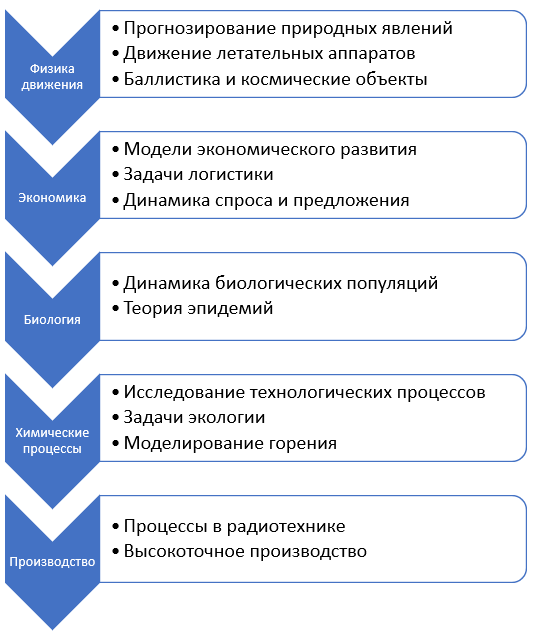
\includegraphics[width=10cm]{2-00-actuality}
    \caption{Области применения ОДУ}
    \label{fig:actuality}
\end{figure}

Для численного моделирования тех или иных процессов нужно использовать специализированные программы и библиотеки, которых на
сегодняшний день предоставлено большое количество, однако все они имеют свои ограничения и недостатки. % Основная часть
    \section{ЦЕЛЬ И ЗАДАЧИ РАБОТЫ} %поменять с программами местами

\textit{Целью} работы является создание комплекса программ для решения ОДУ и СДУ и её дальнейшая отладка на модельных задачах.
Безусловно, в этот программный комплекс должны входить различные явные и неявные методы решения ОДУ, графический
пользовательский интерфейс, парсер математических выражений и многое другое.

В связи с этим можно сформулировать следующие задачи, представленные на рисунке \ref{fig:goals}:
\begin{itemize}
    \item выполнить обзор существующих программ для решения ОДУ, выявить их основные недостатки;
    \item реализовать стандартный набор явных, неявных, вложенных, диагональных, а так же многошаговых методов решения ОДУ;
    \item разработать парсер математических выражений, который можно использовать для ввода задачи Коши. Адаптировать парсер для
    применения его в задачах химической кинетики, в частности для ввода химических компонент, химических реакций, скоростей
    химических реакций и другой информации, необходимой для моделирования химической кинетики;
    \item разработка графического пользовательского интерфейса, дизайна программы и инструментов для генерации pdf-отчётов о решениях
    задач;
    \item выбрать оптимальные по времени и точности схемы для моделирования различных химических процессов на основе разработки ПО
    для решения систем ОДУ явными и неявными методами;
    \item сравнение с существующими программами для решения ОДУ и СДУ.
\end{itemize}

После выполнения данных задач, можно приступить к разработке отдельных модулей для работы с задачами физики, биологии и т.д. Так же
планируется работа над кроссплатформенностью.

\begin{figure}
    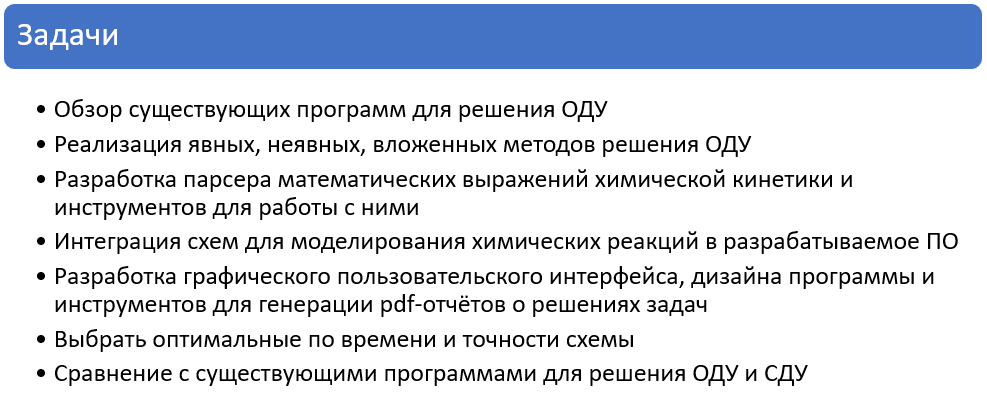
\includegraphics[width=15cm]{2-02-goals}
    \caption{Основные задачи проекта}
    \label{fig:goals}
\end{figure}

Идея работы, основные элементы алгоритмов и результаты тестовых испытаний были изложены 11 апреля 2023 г. на 49-й конференции
Гагаринских чтений
по направлению №7 ("Математические методы в аэрокосмической науке и технике")
секции №3 ("Теоретическая механика и дифференциальные уравнения"). Темой доклада было "Моделирование и оптимизация химической кинетики
на базе схем Рунге-Кутты для решения жёстких систем ОДУ". Тезисы доклада будут опубликованы в сборнике трудов.

Так же была подана заявка на участие в 23-й международной конференции по вычислительной механике и современным прикладным
программным системам (ВМСППС'2023) с темой “Моделирование жёстких систем дифференциальных уравнений на базе схем Рунге-Кутты”,
которая будет проводиться с 4 по 13 сентября 2023 г. 
    \section{ПРОГРАММЫ И БИБЛИОТЕКИ ДЛЯ РЕШЕНИЯ ОДУ}

Программ для решения ОДУ достаточно много. На рисунке \ref{fig:programs} приведены
некоторые популярные программы и библиотеки для решения дифференциальных
уравнений. Рассмотрим детально достоинства и недостатки каждой из них.

\begin{figure}
    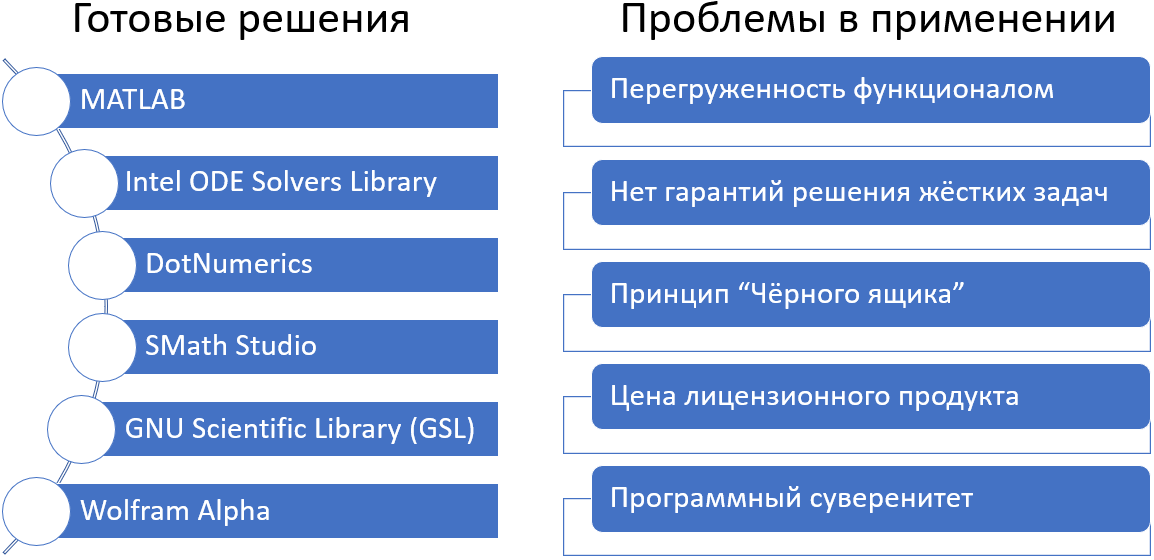
\includegraphics[width=15cm]{2-01-programs}
    \caption{Программы и библиотеки}
    \label{fig:programs}
\end{figure}

Наиболее распространённый программный продукт ~--- пакет программ для решения задач технических вычислений MATLAB. Первый выпуск состоялся в 1984 году. Пакет используют
более миллиона инженерных и научных работников, он работает на большинстве современных операционных систем, включая Linux, macOS и
Windows. Разработчиком является американская компания The MathWorks. Написан с использованием языков программирования С, С++, Fortran,
Java.

Для решения ОДУ MATLAB предлагает следующие функции:
\begin{itemize}
    \item ode23() ~--- метод решения нежёстких дифференциальных уравнений; метод низкого порядка,
    \item ode45() ~--- метод решения нежёстких дифференциальных уравнений; метод среднего порядка,
    \item ode113() ~--- метод решения нежёстких дифференциальных уравнений; метод переменного порядка,
    \item ode15s() ~--- метод решения жёстких дифференциальных уравнений; метод переменного порядка,
    \item ode23s() ~--- метод решения жёстких дифференциальных уравнений; метод низкого порядка.
\end{itemize}

MATLAB имеет свой собственный язык программирования для подготовки данных и большую библиотеку для работы с матрицами, построения
графиков и численных вычислений. Однако он является довольно тяжёлым, имеет низкую скорость работы и не
подходит для решения задач химической кинетики. Помимо этого, в бесплатной версии недостаточно инструментов, а цена полной версии
несолько завышена.

Альтернативу пакету MATLAB может составить отечественная программа SMath Studio, разработанная ООО "ЭсМат".
SMath Studio предназначена для вычисления математических выражений и построения графиков функций. Бета-версия была выпущена в 2018
году и работа над обновлениями продолжается в настоящее время. Работа с интерфейсом
программы напоминает работу с обычным листом бумаги, так как все математические выражения в ней записываются не в строчку текстом,
а в графическом, удобном для человека, виде (по аналогии с системой Mathcad).

Для решения ОДУ в SMath Studio реализованы следующие методы:

\begin{itemize}
    \item неявный метод Эйлера (2-го порядка),
    \item явный метод Рунге-Кутты (классический 4-го порядка).
\end{itemize}

Ограниченное количество методов для решения ОДУ не позволяет использовать её для решения жёстких задач и задач химичесой кинетики
в частности.

В дополнение предыдущей программы можно посмотреть библиотеку Intel ODE Solver Library.
Библиотека написана на языке C со всеми вытекающими отсюда зависимостями. Доступны 32- и 64-разрядные версии.

В этой библиотеке следует выделить следующие программы и функции:
\begin{itemize}
    \item rkm9st() ~--- функция для решения нежёстких и средне-жёстких систем ОДУ с использованием явного метода, который основан на
        методе Мерсона 4-го порядка и многоступенчатом методе 1-го порядка, включающем до 9 этапов с контролем устойчивости,
    \item mk52lfn() ~--- специализированная процедура для решения жёстких систем ОДУ с использованием неявного метода, основанного
        на L-стабильном (5,2)-методе с числовой матрицей Якоби, которая вычисляется с помощью процедуры,
    \item mk52lfa() ~--- специализированная программа для решения жёстких систем ОДУ с использованием неявного метода, основанного на
        L-stable (5,2)-методе с численным или аналитическим вычислением матрицы Якоби. Пользователь должен предоставить процедуру для
        этого вычисления,
    \item rkm9mkn() ~--- специализированная процедура для решения систем ОДУ с переменной или априори неизвестной жёсткостью;
        автоматически выбирает явную или неявную схему на каждом шаге и при необходимости вычисляет числовую матрицу Якоби,
    \item rkm9mka() ~--- специализированная подпрограмма для решения систем ОДУ с переменной или априори неизвестной жёсткостью;
        автоматически выбирает явную или неявную схему на каждом шаге. Пользователь должен предоставить процедуру для численного или
        аналитического вычисления матрицы Якоби.
\end{itemize}

У данной библиотеки есть хороший набор для решения нежёстких задач, есть автоматический выбор явного или неявного шага на каждой
итерации, однако для решения жёстких задач требуется дополнительно вводить Якобиан, что достаточно проблематично.

GNU Scientific Library (или GSL) ~--- это библиотека, написанная на языке программирования C для численных вычислений в прикладной
математике и науке. GSL является частью проекта GNU (Массачусетский технологический институт, США) и распространяется на условиях
лицензии GPL.
Первый релиз состоялся в 1996 году.

GSL используется, в частности, в таком программном обеспечении, как PSPP и Perl Data Language.

Следует отметить следующие достаточно хорошо известные явные методы:
\begin{itemize}
    \item rk2() ~--- явный метод Рунге-Кутты (2, 3),
    \item rk4() ~--- явный 4-й порядок (классический) Рунге-Кутты. Оценка погрешности осуществляется методом удвоения шага,
    \item rkf45() ~--- явный метод Рунге-Кутты-Фельберга (4, 5),
    \item rkck() ~--- явный метод Рунге-Кутты Кэш-Карпа (4, 5),
    \item rk8pd() ~--- явный метод Рунге-Кутты Принца-Дорманда (8, 9).
\end{itemize}

Среди неявных методов можно отметить методы, требующие построение Якобиана до 4-го порядка и большой набор многошаговых методов типа
Адамса:
\begin{itemize}
    \item rk1imp() ~--- неявный гауссовский метод Рунге-Кутты первого порядка. Также известен как неявный метод Эйлера или обратный
        метод Эйлера. Оценка погрешности осуществляется методом удвоения шага. Для этого алгоритма требуется якобиан,
    \item rk2imp() ~--- неявный гауссовский метод Рунге-Кутты второго порядка. Также известно как неявное правило средней точки. Оценка
        погрешности осуществляется методом удвоения шага. Для этого шагового двигателя требуется якобиан,
    \item rk4imp() ~--- неявный гауссов Рунге-Кутта 4-го порядка. Оценка погрешности осуществляется методом удвоения шага. Для этого
        алгоритма требуется якобиан,
    \item bsimp() ~--- неявный метод Булирша-Стоера (многошаговый). Этот метод, как правило, подходит для сложных задач. Для этого
        шагового двигателя требуется якобиан,
    \item msadams() ~--- линейный многоступенчатый метод Адамса с переменным коэффициентом в форме Nordsieck. Этот шаговый процессор
        использует явные методы Адамса-Башфорта (предсказатель) и неявные методы Адамса-Моултона (корректор) в режиме функциональной
        итерации $P(EC)^m$. Порядок методов динамически варьируется от 1 до 12,
    \item msbdf() ~--- метод линейной многоступенчатой формулы обратного дифференцирования с переменным коэффициентом (BDF) в форме
        Nordsieck. Этот шаговый преобразователь использует явную формулу BDF в качестве предиктора и неявную формулу BDF в качестве
        корректора. Для решения системы нелинейных уравнений используется модифицированный итерационный метод Ньютона. Порядок методов
        динамически варьируется от 1 до 5. Этот метод, как правило, подходит для сложных задач. Для этого шагового двигателя требуется
        якобиан.
\end{itemize}

В данной библиотеке большое количество как явных, так и неявных методов, но для невных методов как и в библиотеке Intel ODE Solver
Library требуется самостоятельное вычисление Якобиана. Недостаток именно библиотечного вида заключается в том, что надо писать модули
обращения и модули обработки результата.

Следующей библиотекой для рассмотрения является DotNumerics. Она включает в себя числовую библиотеку для .NET. Библиотека написана на
чистом C\# и содержит более 100 000 строк кода с
самыми передовыми алгоритмами для линейной алгебры, дифференциальных уравнений и задач оптимизации. Библиотека линейной алгебры
включает CSLapack, Cabelas и CSEispack, эти библиотеки являются переводом с Fortran на C\# LAPACK, BLAS и EISPACK соответственно.

Основные решатели для нежёстких систем:
\begin{itemize}
    \item ExplicitRK45() ~--- решает задачу с начальными значениями для нелинейных обыкновенных дифференциальных уравнений, используя
        явный метод Рунге-Кутты порядка (4)5,
    \item AdamsMoulton() ~--- решает начальную задачу для нелинейных обыкновенных дифференциальных уравнений с использованием метода
        Адамса-Моултона.
\end{itemize}

Решатели для жёстких систем:
\begin{itemize}
    \item ImplicitRK5() ~--- решает начальную задачу для жёстких обыкновенных дифференциальных уравнений с использованием неявного
        метода Рунге-Кутты порядка 5,
    \item GearsBDF() ~--- решает начальную задачу для жёстких обыкновенных дифференциальных уравнений с использованием многошагового
        метода BDF Gear.
\end{itemize}

В данной библиотеке представлено небольшое число методов решения ОДУ до 5 порядка точности. В основном эта библиотека обслуживает
не только задач дифференциальных уравнений, но и задачи линейной алгебры, в том числе задачи оптимизации, поэтому она содержит мало методов
для решения моей задачи.

Отметим так же систему Wolfram Alpha. Это база знаний и набор вычислительных алгоритмов, вопросно-ответная
система.

Wolfram Alpha способен переводить данные между различными единицами
измерения, системами счисления, подбирать общую формулу последовательности, находить возможные замкнутые формы для приближенных
дробных чисел, вычислять суммы, пределы, интегралы, решать уравнения и системы уравнений, производить операции с матрицами, определять
свойства чисел и геометрических фигур. Отдельного внимания стоит парсинг математических выражений.

В частности система Wolfram Alpha способна решать ОДУ стандартными явными методами:
\begin{itemize}
    \item метод Эйлера (2-го порядка),
    \item метод средних точек, модифицированный метод Эйлера,
    \item метод Хойна, вариант модифицированного метода Эйлера,
    \item метод Рунге-Кутты 3-го порядка,
    \item метод Рунге-Кутты (классический 4-го порядка),
    \item метод Рунге-Кутты-Фалберга,
    \item метод Дормана-Принца.
\end{itemize}

Система Wolfram Alpha является облачной. Это означает, что для работы с ней необходимо постоянное подключение к интернету. Ещё
одним недостатком является наличие платного функционала и отсутствие готовых модулей для создания и решения СДУ химической кинетики.

Несмотря на большое число программ и библиотек для решение ДУ, появилась потребность в создании программы (с большим выбором расчетных
схем) для решения (в то числе и) жёстких систем ДУ для задач химической кинетики.
    \section{КЛАССИЧЕСКИЕ МЕТОДЫ ДЛЯ РЕШЕНИЯ ОДУ}

\subsection{Постановка задачи}

Программа, над которой ведётся работа, предназначена для решения дифференциальных уравнений или систем дифференциальных 
уравнений с начальными значениями, то есть задачи Коши ~--- классической математической постановки. 
Сама по себе задача достаточно сложная и изучалась уже более ста лет.

Конкретная прикладная задача сводится к решению дифференциального уравнения произвольного порядка \ref{eq-koshi}:
\begin{equation}
    \begin{cases}
        y^{(n)} = f(x, y, y', y'', ..., y^{(n - 1)})\\
        y(x_0) = y_0\\
        y'(x_0) = y_1\\
        y''(x_0) = y_2\\
        ...\\
        y^{(n - 1)}(x_0) = y_{n - 1}
    \end{cases}
    \label{eq-koshi}
\end{equation}

Данное уравнение произвольного порядка $n$ может быть преобразовано в систему из $n$ дифференциальных уравнений первого порядка путём
замены переменных. Пример \ref{eq-koshi-system} демонстрирует преобразование задачи Коши второго порядка в систему из 2-х уравнений
первого порядка, путём замены $y'$ на $z$:
\begin{equation}
    \begin{cases}
        z' = f(x, y, y', y'')\\
        y' = z\\
        y(x_0) = y_0\\
        z(x_0) = y_1
    \end{cases}
    \label{eq-koshi-system}
\end{equation}

Из курса дифференциальных уравнений известно, что задача с начальными условиями при непрерывных правых частях, удовлетворяющих условию
Липшица по всем переменным, имеет единственное решение.

Методы решения дифференциальных уравнений можно классифицировать на точные, приближенные и численные. Точные методы, которые изучаются
в курсе дифференциальных уравнений и могут быть применены к очень ограниченному кругу уравнений, позволяют выразить решение
дифференциальных уравнений либо через элементарные функции, либо с помощью квадратур от элементарных функций. К приближенным методам
относятся приемы, в которых решение дифференциального уравнения получается, как предел некоторой последовательности, элементы которой
построены с помощью элементарных функций. Численные методы представляют собой алгоритмы вычисления приближенных значений искомой
функции в узлах. %ссылку бы сюда

Такие задачи могут отличаться между собой сложностью решения. Так одни задачи можно решать при помощи группы явных методов и получать
достаточно точное решение. Другие же задачи, в которых присутствует резкий скачок градиента функции, решать приходится с использованием
неявных схем. Такие задачи называются жёсткими.

\subsection{Жёсткость}

Будем считать линейную систему обыкновенных дифференциальных уравнений $u' = Au$ ($A$ ~--- постоянная матрица $n \times n$)
жёсткой, если выполняются следующие требования:

\begin{enumerate}
    \item все собственные числа $\lambda_i$ матрицы $A$ имеют отрицательную действительную часть, т. е. $Re\lambda_i < 0$, 
    $i = 1, 2, ..., n$;
    \item число
        \begin{equation}
            S = \dfrac{\max\limits_{1 \leq k \leq n}|Re\lambda_k|}{\min\limits_{1 \leq k \leq n}|Re\lambda_k|}
            \label{eq:tough}
        \end{equation}
        велико
\end{enumerate}

Число \ref{eq:tough} называется жёсткостью задачи.

Для жёстких задач число жёсткости должно быть намного больше единицы, однако чёткой границы между жёсткой и нежёсткой задачей нет. Так
модельные уравнения с числом жёсткости более $100$ уже дают небольшие скачки погрешности решения. В задачах химической кинетики число
жёсткости может быть более $10^6$.

\subsection{Явные схемы для решения ОДУ}

Для решения жёстких и нежёстких задач можно использовать различные семейства методов. В данной работе будет рассмотрено семейство
одношаговых методов Рунге-Кутты.

В семейство методов Рунге-Кутты входит огромное число схем, как явных, так и неявных. Все эти методы представлены в виде таблиц
Бутчера. Общий вид явных схем представлен на рисунке \ref{fig:Runge}.

Явные методы обладают нижней диагональной формой таблицы Бутчера и позволяют решать задачи обычными маршевыми методами. В связи с тем,
что явные методы являются условно устойчивыми, работа с ними сильно зависит от размера шага итегрирования и для достижения заданной
точности требуют достаточно мелкий шаг интегрирования и повторного вычисления для повышения порядка точности процедурой Рунге-Ромберга.

%Общий вид явных схем:

% \begin{equation}
%     \begin{cases}
%         y_{k + 1} = y_k + \Delta y_k\\
%         \Delta y_k = \mathlarger{\sum}\limits_{i = 1}^{p}b_iK_i^k\\
%         K_i^k = hf\underset{i = 2, 3, ..., p}{(x_k + c_i h, y_k + h \mathlarger{\sum}\limits_{j = 1}^{i - 1}a_{ij}K_j^k)}
%     \end{cases}
%     \label{eq:explicit}
% \end{equation}

\begin{figure}
    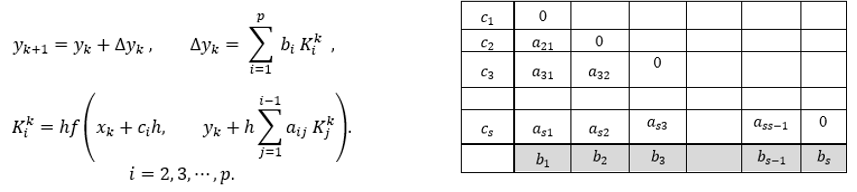
\includegraphics[width=15cm]{2-03-runge}
    \caption{Общий вид явных схем}
    \label{fig:Runge}
\end{figure}

Примеры таблиц Бутчера \ref{tab:RungeKutta4}, \ref{tab:RungeKutta6} для явных методов:

\begin{table}    
    \caption{Таблица Бутчера для метода явного метода Рунге-Кутты 4-го порядка}
    \begin{tabular}{|c|c|c|c|c|}
    \hline
    $0$ & $0$ & $0$ & $0$ & $0$\\
    \hline
    $\frac{1}{2}$ & $\frac{1}{2}$ & $0$ & $0$ & $0$\\
    \hline
    $\frac{1}{2}$ & $0$ & $\frac{1}{2}$ & $0$ & $0$\\
    \hline
    $1$ & $0$ & $0$ & $1$ & $0$\\
    \hline
    $0$ & \cellcolor{lightgray} $\frac{1}{6}$ & \cellcolor{lightgray} $\frac{1}{3}$ & \cellcolor{lightgray} $\frac{1}{3}$ & \cellcolor{lightgray} $\frac{1}{6}$\\
    \hline
    \end{tabular}
    \label{tab:RungeKutta4}
\end{table}

\begin{table}    
    \caption{Таблица Бутчера для метода явного метода Рунге-Кутты 6-го порядка}
    \begin{tabular}{|c|c|c|c|c|c|c|}
    \hline
    $0$ & $0$ & $0$ & $0$ & $0$ & $0$ & $0$\\
    \hline
    $\frac{1}{4}$ & $\frac{1}{4}$ & $0$ & $0$ & $0$ & $0$ & $0$\\
    \hline
    $\frac{1}{2}$ & $\frac{1}{2}$ & $0$ & $0$ & $0$ & $0$ & $0$\\
    \hline
    $\frac{1}{2}$ & $\frac{1}{7}$ & $\frac{2}{7}$ & $\frac{1}{14}$ & $0$ & $0$ & $0$\\
    \hline
    $\frac{3}{4}$ & $\frac{3}{8}$ & $0$ & $-\frac{1}{2}$ & $\frac{7}{8}$ & $0$ & $0$\\
    \hline
    $1$ & $-\frac{4}{7}$ & $\frac{12}{7}$ & $-\frac{2}{7}$ & $-1$ & $7$ & $0$\\
    \hline
    $0$ & \cellcolor{lightgray} $\frac{7}{90}$ & \cellcolor{lightgray} $\frac{16}{45}$ & \cellcolor{lightgray} $-\frac{1}{3}$ & \cellcolor{lightgray} $\frac{7}{15}$ & \cellcolor{lightgray} $\frac{16}{45}$ & \cellcolor{lightgray} $\frac{7}{90}$\\
    \hline
    \end{tabular}
    \label{tab:RungeKutta6}
\end{table}

\subsection{Явные вложенные схемы для решения ОДУ}

В связи с перечисленными недостатками обычных явных схем, есть смысл применить явные вложенные схемы, которые базируются так же на
нижней треугольной матрице Бутчера, обладают маршевым
методом решения и позволяют на базе одних и тех же поправочных коэффициентов моделировать решение с разным порядком точности и тем
самым либо увеличивать шаг интегрирования, либо уменьшать.

%(примеры таблиц Дормана-Принца и Фалберга 2)
%(формулы в общем виде)

\begin{figure}
    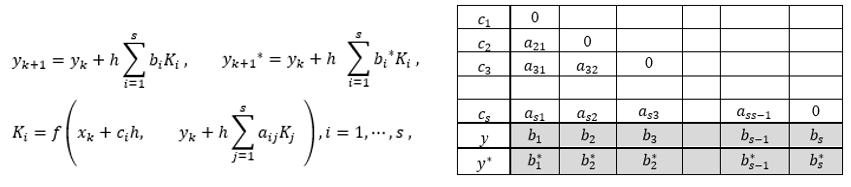
\includegraphics[width=15cm]{2-03-falberg}
    \caption{Общий вид явных вложенных схем}
    \label{fig:Falberg}
\end{figure}

Примеры таблиц Бутчера для вложенных методов:

\begin{table}
    \caption{Таблица Бутчера для метода Фалберга 2-го порядка}
    \begin{tabular}{|c|c|c|c|}
    \hline
    $0$ & $0$ & $0$ & $0$\\
    \hline
    $1$ & $1$ & $0$ & $0$\\
    \hline
    $\frac{1}{2}$ & $\frac{1}{4}$ & $\frac{1}{4}$ & $0$\\
    \hline
    $0$ & \cellcolor{lightgray} $\frac{1}{2}$ & \cellcolor{lightgray} $\frac{1}{2}$ & \cellcolor{lightgray} $0$\\
    \hline
    $0$ & \cellcolor{lightgray} $\frac{1}{6}$ & \cellcolor{lightgray} $\frac{1}{6}$ & \cellcolor{lightgray} $\frac{4}{6}$\\
    \hline
    \end{tabular}
    \label{tab:Falberg2}
\end{table}

\begin{table}    
    \caption{Таблица Бутчера для метода Дормана-Принца 4-го порядка}
    \begin{tabular}{|c|c|c|c|c|c|c|c|}
    \hline
    $0$ & $0$ & $0$ & $0$ & $0$ & $0$ & $0$ & $0$\\
    \hline
    $\frac{1}{5}$ & $\frac{1}{5}$ & $0$ & $0$ & $0$ & $0$ & $0$ & $0$\\
    \hline
    $\frac{3}{10}$ & $\frac{3}{40}$ & $\frac{9}{40}$ & $0$ & $0$ & $0$ & $0$ & $0$\\
    \hline
    $\frac{4}{5}$ & $\frac{44}{45}$ & $-\frac{56}{15}$ & $\frac{32}{9}$ & $0$ & $0$ & $0$ & $0$\\
    \hline
    $\frac{8}{9}$ & $\frac{19372}{6561}$ & $-\frac{25360}{2187}$ & $\frac{64448}{6561}$ & $-\frac{212}{729}$ & $0$ & $0$ & $0$\\
    \hline
    $1$ & $\frac{9017}{3168}$ & $-\frac{355}{33}$ & $\frac{46732}{5247}$ & $\frac{49}{176}$ & $-\frac{5103}{18656}$ & $0$ & $0$\\
    \hline
    $1$ & $\frac{35}{384}$ & $0$ & $\frac{500}{1113}$ & $\frac{125}{192}$ & $-\frac{2187}{6784}$ & $\frac{11}{84}$ & $0$\\
    \hline
    $0$ & \cellcolor{lightgray} $\frac{35}{384}$ & \cellcolor{lightgray} $0$ & \cellcolor{lightgray} $\frac{500}{1113}$ & \cellcolor{lightgray} $\frac{125}{192}$ & \cellcolor{lightgray} $-\frac{2187}{6784}$ & \cellcolor{lightgray} $\frac{11}{84}$ & \cellcolor{lightgray} $0$\\
    \hline
    $0$ & \cellcolor{lightgray} $\frac{5179}{57600}$ & \cellcolor{lightgray} $0$ & \cellcolor{lightgray} $\frac{7571}{16695}$ & \cellcolor{lightgray} $\frac{393}{640}$ & \cellcolor{lightgray} $-\frac{92097}{339200}$ & \cellcolor{lightgray} $\frac{187}{2100}$ & \cellcolor{lightgray} $\frac{1}{40}$\\
    \hline
    \end{tabular}
    \label{tab:DormanPrince4}
\end{table}

\subsection{Неявные схемы для решения ОДУ}

К наиболее сложным методам можно отнести группу неявных схем. Плотно заполненная таблица Бутчера не позволяет использовать маршевые
методы и принуждает решать систему алгебраических уравнений на каждом шаге интегрирования, что вызывет определённые сложности у
разработчиков.

\begin{figure}
    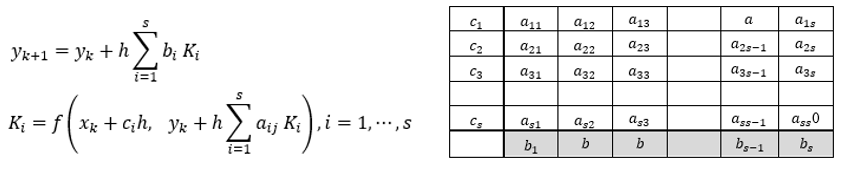
\includegraphics[width=15cm]{2-03-gauss}
    \caption{Общий вид неявных схем}
    \label{fig:Gauss}
\end{figure}

Примеры таблиц Бутчера для неявных методов:

\begin{table}    
    \caption{Таблица Бутчера для метода неявного метода Гаусса 4-го порядка}
    \begin{tabular}{|c|c|c|}
    \hline
    $\frac{1}{2} - \frac{\sqrt{3}}{6}$ & $\frac{1}{4}$ & $\frac{1}{4} - \frac{\sqrt{3}}{6}$\\
    \hline
    $\frac{1}{2} + \frac{\sqrt{3}}{6}$ & $\frac{1}{4} + \frac{\sqrt{3}}{6}$ & $\frac{1}{4}$\\
    \hline
    $0$ & \cellcolor{lightgray} $\frac{1}{2}$ & \cellcolor{lightgray} $\frac{1}{2}$\\
    \hline
    \end{tabular}
    \label{tab:Gauss4}
\end{table}

\begin{table}    
    \caption{Таблица Бутчера для метода неявного метода Гаусса 6-го порядка}
    \begin{tabular}{|c|c|c|c|}
    \hline
    $\frac{1}{2} - \frac{\sqrt{15}}{10}$ & $\frac{5}{36}$ & $\frac{2}{9} - \frac{\sqrt{15}}{15}$ & $\frac{5}{36} - \frac{\sqrt{15}}{30}$\\
    \hline
    $\frac{1}{2}$ & $\frac{5}{36} + \frac{\sqrt{15}}{24}$ & $\frac{2}{9}$ & $\frac{5}{36} - \frac{\sqrt{15}}{24}$\\
    \hline
    $\frac{1}{2} + \frac{\sqrt{15}}{10}$ & $\frac{5}{36} + \frac{\sqrt{15}}{30}$ & $\frac{2}{9} + \frac{\sqrt{15}}{15}$ & $\frac{5}{36}$\\
    \hline
    $0$ & \cellcolor{lightgray} $\frac{5}{18}$ & \cellcolor{lightgray} $\frac{4}{9}$ & \cellcolor{lightgray} $\frac{5}{18}$\\
    \hline
    \end{tabular}
    \label{tab:Gauss6}
\end{table}

Помимо перечисленных групп методов, существуют так же диагональные неявные методы, неявные вложенные, неявные методы без одной строки
или столбца, но все они являются подгруппами неявных методов и используют тот же вид общей схемы.

Преимущество явных методов заключается в производительности, так как им не нужно решать на каждом шаге системы алгебраических
уравнений. Отсюда следует, что использование явных методов даёт больший выигрыш по времени, чем использование более производительного
оборудования и распараллеливания. Главным преимуществом неявных методов является наличие устойчивости (А-устойчивости, L-устойчивости и
так далее), в результате чего полученное ими решение является гарантированно устойчивым, в отличие от явных.

\subsection{Устойчивость}

Текст

Однако некоторые СДУ, описывающие химические процессы можно решить и явными методами с требуемой точностью, потому что свойства А и
L-устойчивости являются
лишь достаточным, но не необходимым условием эффективности решения, поэтому нельзя использовать только те или иные методы. Выбрать
оптимальный метод можно путём целевого тестирования.


%Цитирование источника 4 \cite{Wikipedia4} \cite{cite_1_2} \cite{cite_1_15} \cite{cite_1_16}.

    \section{РЕАЛИЗАЦИЯ}

Проанализировав все вышеперечисленные программы 

Таким образов в программу вошли классические алгоритмы численных методов, такие как методы матричной алгебры, методы
Ньютона и так далее. Для её написания были использованы \textit{язык программирования C++}, \textit{фреймворк QT} и система сборки
проектов \textit{CMake} \ref{fig:stack}.
Для поиска ошибок и утечек памяти применилась связка из отладчика \textit{GDB} и профилировщика \textit{Valgrind}. 

\begin{figure}
    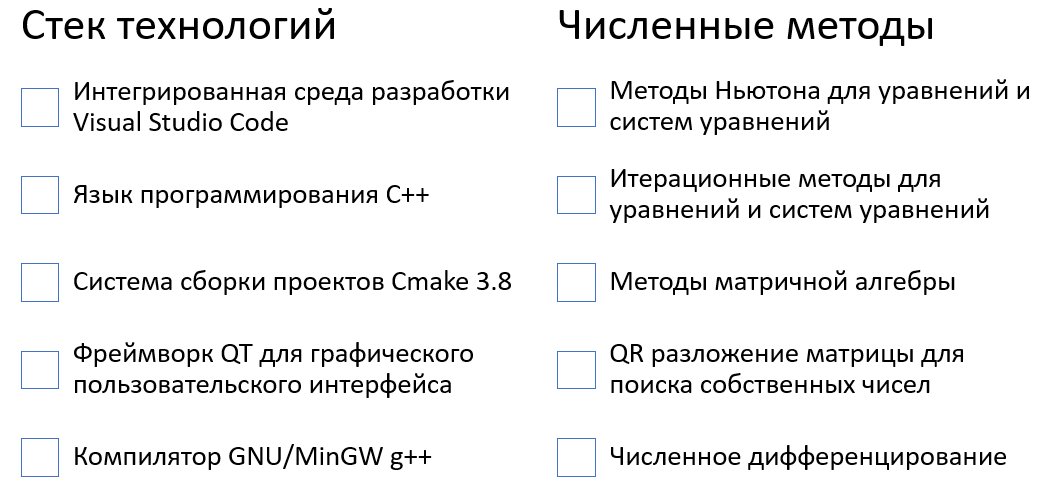
\includegraphics[width=15cm]{2-04-realisation}
    \caption{Технологии и алгоритмы}
    \label{fig:stack}
\end{figure}

В данной программе реализован большой перечень как явных так и неявных методов с различным порядком точности.

%Для повышения порядка точности явных методов используется процедура Рунге-Ромберга, заключающаяся в повторном решении в точке с вдвое меньшим шагом и сравнении с предыдущим.

%Если погрешность сильно меньше заданной точности, что шаг интегрирования стоит уменьшить, если же больше, что увеличить.

%и вложенные методы. Неявные и их виды ()нулевая строка, нулевой столбец, диагональные, полные) параллельные

\textbf{Вычисление жёсткости}

Коэффициентом жёсткости задачи называется отношение максимального модуля действительной части собственных чисел матрицы системы к
минимальной при условии, что все действительные части собственных чисел меньше нуля.

Для вычисления коэффициента жёсткости сначала по данной задаче строится матрица-система. Собственные числа данной матрицы находятся
при помощи алгоритма QR-разложения.

дополнительные методы ()кью-ар
методы решения слау

%методы решения

Для неявных методов используются алгоритмы итераций Ньютона, Зейделя и простой итерации.

%алгоритмы работы с матрицами

Кью-Ар разложение 

хоть метод ньютона и второго порядка но применим и для методов

\textbf{Описание работы программы}

%картинка стека технологий

\textbf{Парсер математических выражений}

При режиме работы с задачей Коши от пользователя требуется ввести задачу и аналитическое решение (при наличии). 

Для обработки строки с задачей используется парсер математических выражений. Проводится лексический анализ строки и строится дерево
математических выражений, содержащее функции в качестве узлов и числовые константы с переменными в качестве листьев. Интерфейс парсера
позволяет использовать его как функтор, принимающий либо одну переменную, либо массив переменных. 

%Далее последует выбор метода решения и точности. В результате работы генерируется pdf-отчёт с краткой постановкой задачи, подробным
%описанием метода решения и таблицы Бутчера, используемой методом, В конце отчёта представлен график с сравнением точного и численного
%решения.

%лексический анализ, жёсткость, выбор метода, построение методов.
%сравнение по времени лексического анализа и встроенных функций
%скрины интерфейса

%==================================

%Программа представляет из себя набор модулей

%форма для вывода/ввода

    \section{ТЕСТИРОВАНИЕ И ВЕРИФИКАЦИЯ ЧИСЛЕННОЙ МОДЕЛИ}

В данном разделе представлены результаты тестирования разработанного численного алгоритма. Основное внимание уделено исследованию точности и производительности метода в зависимости от параметров дискретизации, а также сравнению полной и параболизированной постановок уравнений. Для сравнения точности были выбраны расчёты из~\cite{book11_tur}.

\subsection{Зависимость точности решения от шага дискретизации}

Сравнение проводилось для трёх случаев $H_1 = 0.0150, H_2 = 0.0075, H_3 = 0.0037$. Результаты проверялись по значениям переменной $U$. Входные данные сохранены в фалйе \texttt{test7.py} на GitHub репозитории проекта (ссылка в приложении).

Для анализа влияния шага дискретизации на точность решения была рассмотрена модельная задача о ламинарной струе с химическими реакциями. Исследование проводилось при различных значениях шага по пространству $\Delta x, \Delta y$ и времени $\Delta t$. Как видно из рисунках~\ref{fig:acc_1_1},~\ref{fig:acc_1_2},~\ref{fig:acc_2_1},~\ref{fig:acc_2_2},~\ref{fig:acc_3_1},~\ref{fig:acc_3_2}, уменьшение шага приводит к монотонному снижению погрешности до некоторого предельного значения. 

\begin{figure}
    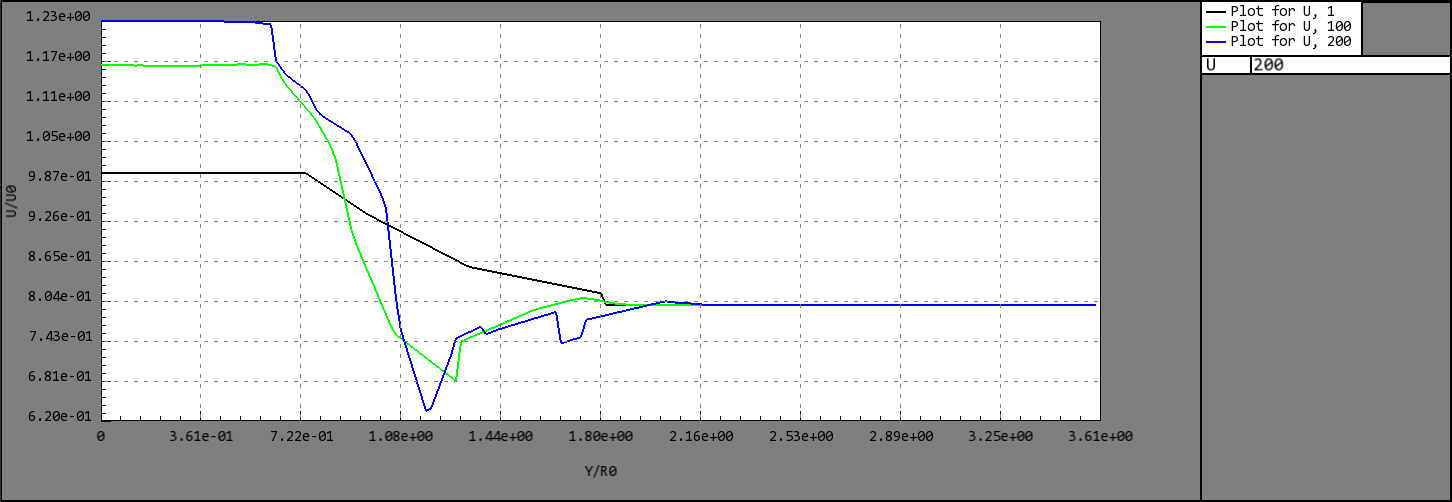
\includegraphics[width=15cm]{2-05-test1}
    \caption{Значение шага $0.015$, параболизованная система}
    \label{fig:acc_1_1}
\end{figure}

\begin{figure}
    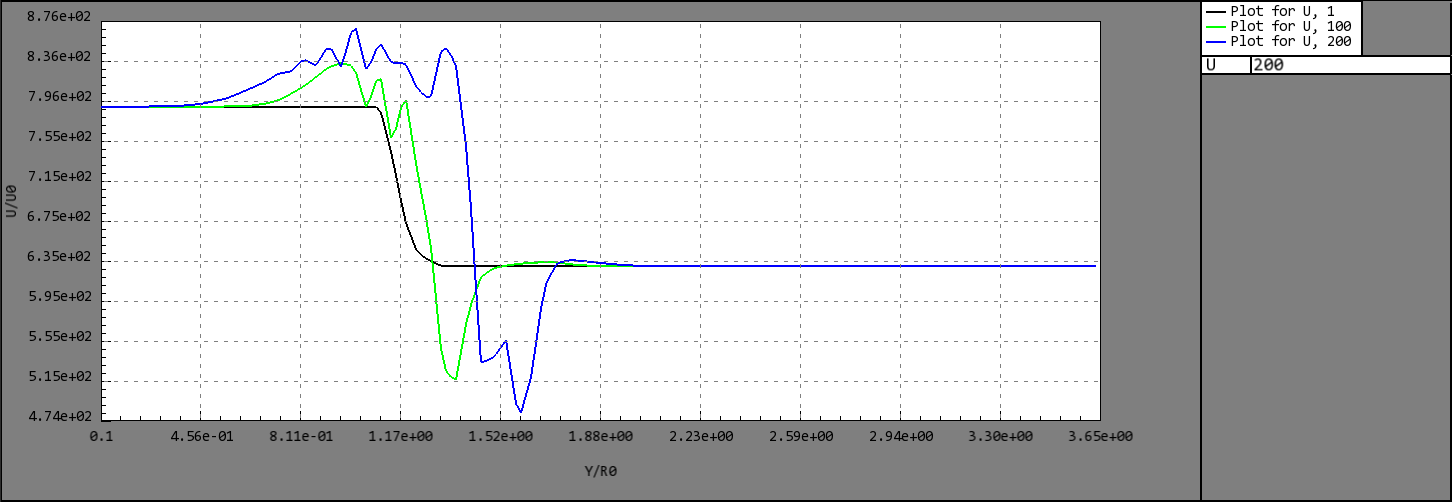
\includegraphics[width=15cm]{2-05-test4}
    \caption{Значение шага $0.015$, полная система}
    \label{fig:acc_1_2}
\end{figure}

\begin{figure}
    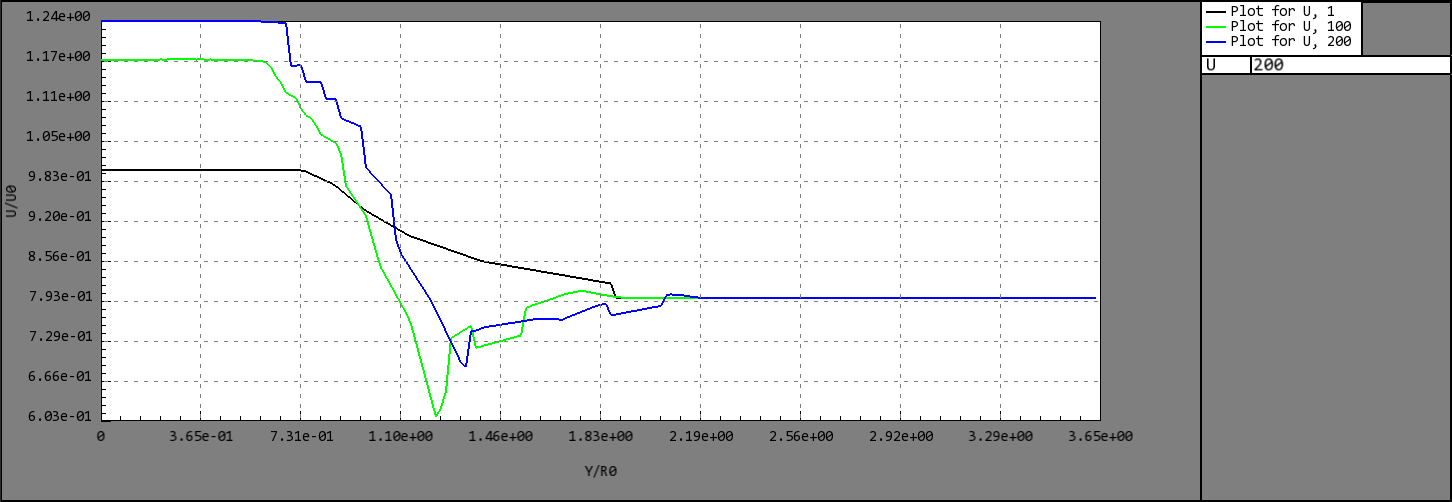
\includegraphics[width=15cm]{2-05-test2}
    \caption{Значение шага $0.0075$, параболизованная система}
    \label{fig:acc_2_1}
\end{figure}

\begin{figure}
    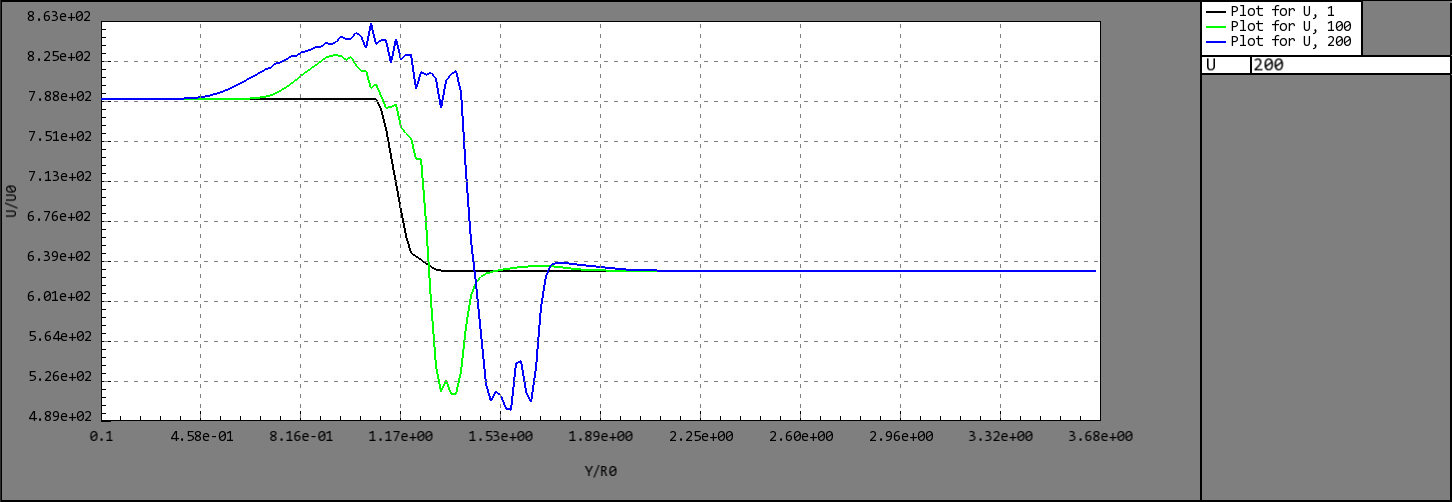
\includegraphics[width=15cm]{2-05-test5}
    \caption{Значение шага $0.0075$, полная система}
    \label{fig:acc_2_2}
\end{figure}

\begin{figure}
    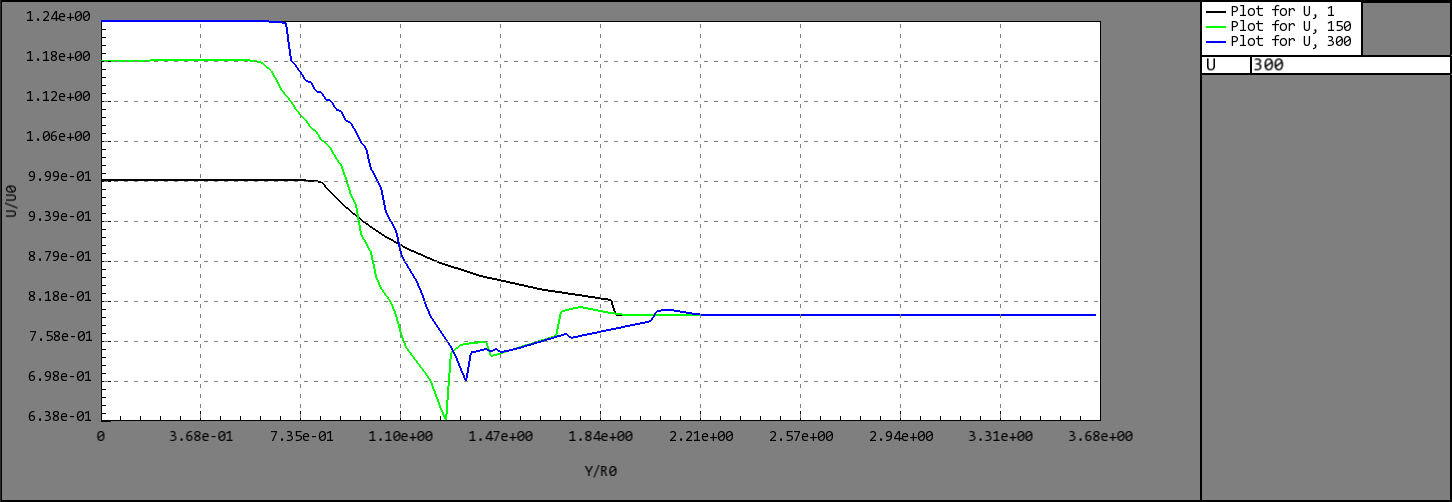
\includegraphics[width=15cm]{2-05-test3}
    \caption{Значение шага $0.0037$, параболизованная система}
    \label{fig:acc_3_1}
\end{figure}

\begin{figure}
    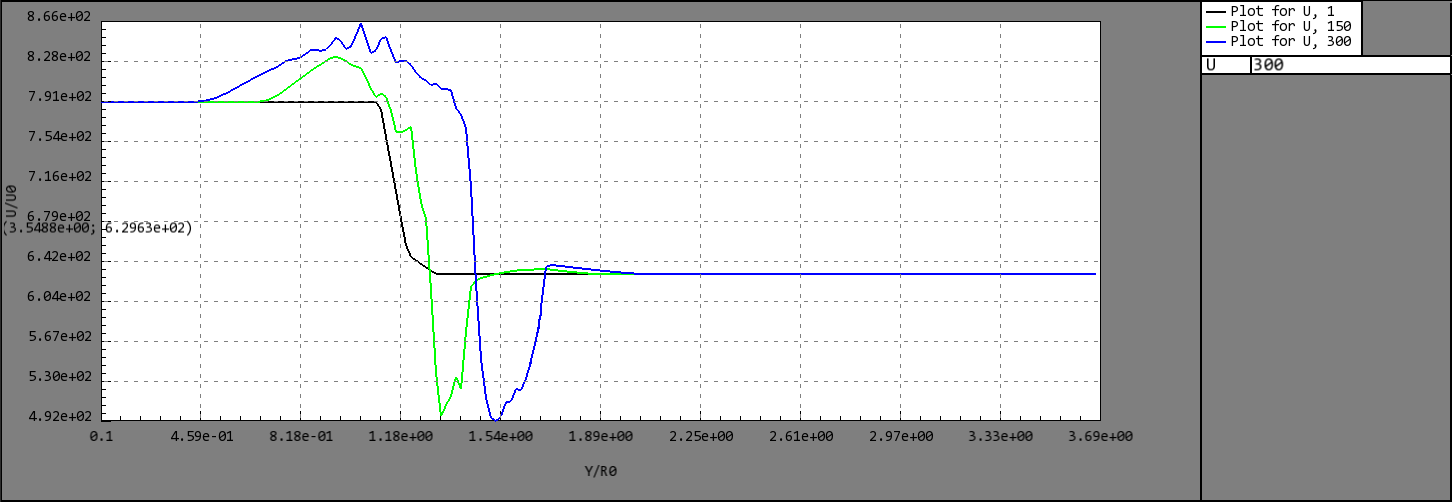
\includegraphics[width=15cm]{2-05-test6}
    \caption{Значение шага $0.0037$, полная система}
    \label{fig:acc_3_2}
\end{figure}

Наблюдаются две характерные области:

\begin{itemize}
\item При $H > 0.007L$ доминирует погрешность аппроксимации
\item При $H < 0.003$ основную роль играют ошибки округления
\end{itemize}

Оптимальным с точки зрения точности и вычислительных затрат оказался шаг $H \approx 0.003$.

\subsection{Сравнение полной и параболизированной систем уравнений}

Для оценки адекватности параболизированной постановки проведено сравнение с полной системой уравнений Навье-Стокса на тестовой задаче о турбулентной струе. Основные результаты представлены в таблице~\ref{tab:comparison}.

\begin{table}[h]
\centering
\caption{Сравнение характеристик течения для разных постановок}
\label{tab:comparison}
    \begin{tabular}{|l|c|c|}
    \hline
    Параметр & Полная система & Параболизированная \\ \hline
    Длина факела, м & 1.25 & 1.31 \\ 
    Макс. температура, K & 2150 & 2095 \\
    Время расчёта, с & 347.9 & 125.6 \\ \hline
    \end{tabular}
\end{table}

Наибольшие расхождения (до 12\%) наблюдаются в зоне обратных течений, где параболизированная постановка менее точна. Однако для основной зоны струи различия не превышают 5\%.

\subsection{Зависимость времени расчёта от шага дискретизации}
\label{subsec:performance}

Производительность алгоритма исследовалась на сетках различной плотности. Результаты представлены на рисунке~\ref{fig:performance}.

\begin{figure}
\centering
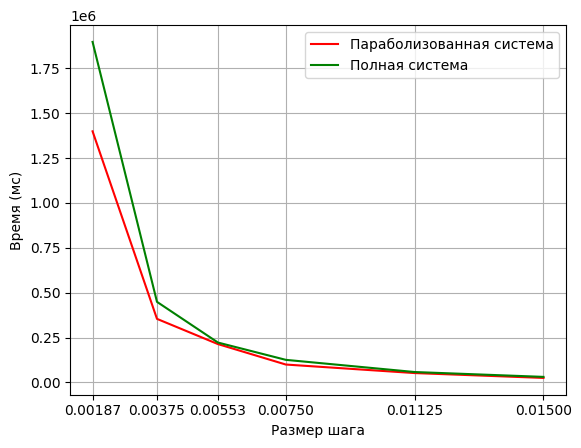
\includegraphics[width=0.8\linewidth]{2-05-time}
\caption{Зависимость времени расчёта от размера шага}
\label{fig:performance}
\end{figure}

Зависимость времени расчёта $T$ от размера шага $H$ хорошо аппроксимируется степенной функцией:
\begin{equation}
T(N) = aN^b
\end{equation}
где $b \approx 1.8$ для параболизированной и $b \approx 2.1$ для полной системы. Уменьшение показателя степени связано с эффективностью маршевого алгоритма.

\subsection{Прочие примеры}

Для демонстрации изменения различных переменных были выбраны следующие начальные данные и размеры шагов (Рис.~\ref{src:format}). Данный формат используется для всех тестовых случаев.

\begin{figure}
\begin{lstlisting}[language=Python, escapeinside=``]
    #R0
    0.01
    #конечный расчёт X - n*R_0
    100
    #конечный расчёт Y - n*R_0
    370
    #размер сетки
    200 500
    #размер профиля
    37
    #путь к базе данных для хим. кинетики
    ./../../test/ChemicTest/bufermm1.txt
    #значения внутри
    5
    U 790
    T 237
    P 50290
    MU 0.18e-4
    Y 1
    #количество переменных с ненулевым профилем
    6
    Y       U       V       W       T       P
    0.100   1.000   0.000   0.000   1.000   1.000
    0.200   1.000   0.000   0.000   1.000   1.000
    0.300   1.000   0.000   0.000   1.000   1.000
    0.400   1.000   0.000   0.000   1.000   1.000
    0.500   1.000   0.000   0.000   1.000   1.000
    0.600   1.000   0.000   0.000   1.000   1.000
    0.700   1.000   0.000   0.000   1.000   1.000
    0.800   1.000   0.000   0.000   1.000   1.000
    0.900   1.000   0.000   0.000   1.000   1.000
    1.000   1.000   0.000   0.000   1.000   0.455
\end{lstlisting}
\caption{Формат входных файлов}
\label{src:format}
\end{figure}

Результаты отображены на рисунках~\ref{fig:acc_U},\ref{fig:acc_V},\ref{fig:acc_MU},\ref{fig:acc_J},\ref{fig:acc_T},\ref{fig:acc_P},\ref{fig:acc_RHO}. Как можно заметить, даже при мелком шаге в расчётах присутствуют некоторые неточности и скачки. Это может быть вызвано неточной моделью турбулентности или издержками параболизации. В дальнейшем можно реализовать более точные модели и заняться более детальной оптимизацией.

\begin{figure}
    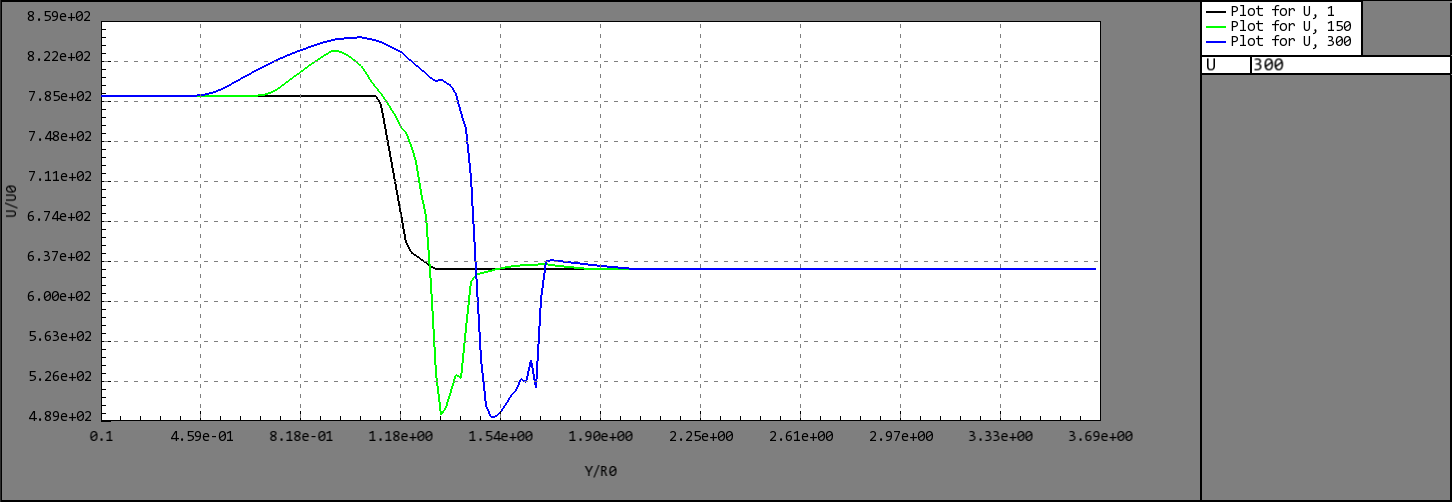
\includegraphics[width=15cm]{2-05-test-U}
    \caption{Значения скорости $U$}
    \label{fig:acc_U}
\end{figure}

\begin{figure}
    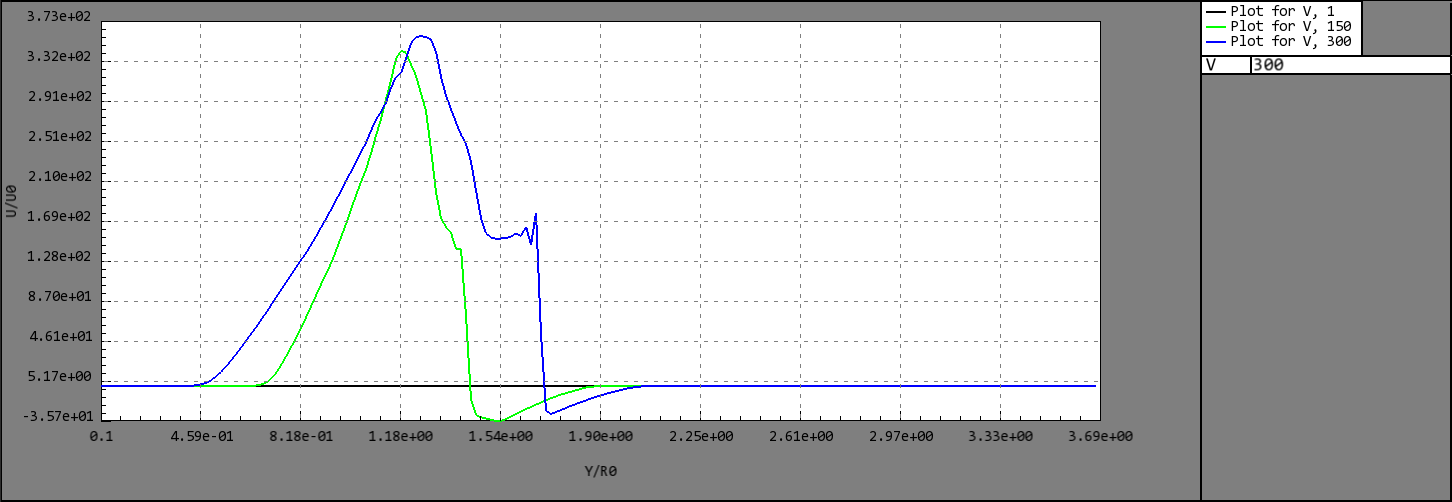
\includegraphics[width=15cm]{2-05-test-V}
    \caption{Значения скорости $V$}
    \label{fig:acc_V}
\end{figure}

\begin{figure}
    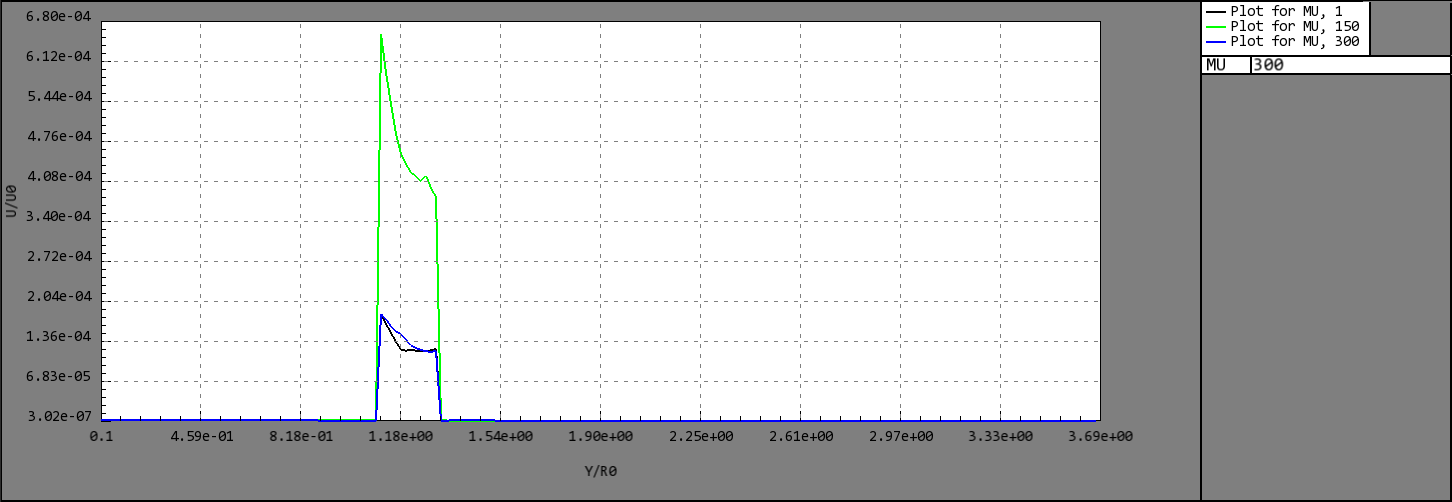
\includegraphics[width=15cm]{2-05-test-MU}
    \caption{Значения вязкости $\mu$}
    \label{fig:acc_MU}
\end{figure}

\begin{figure}
    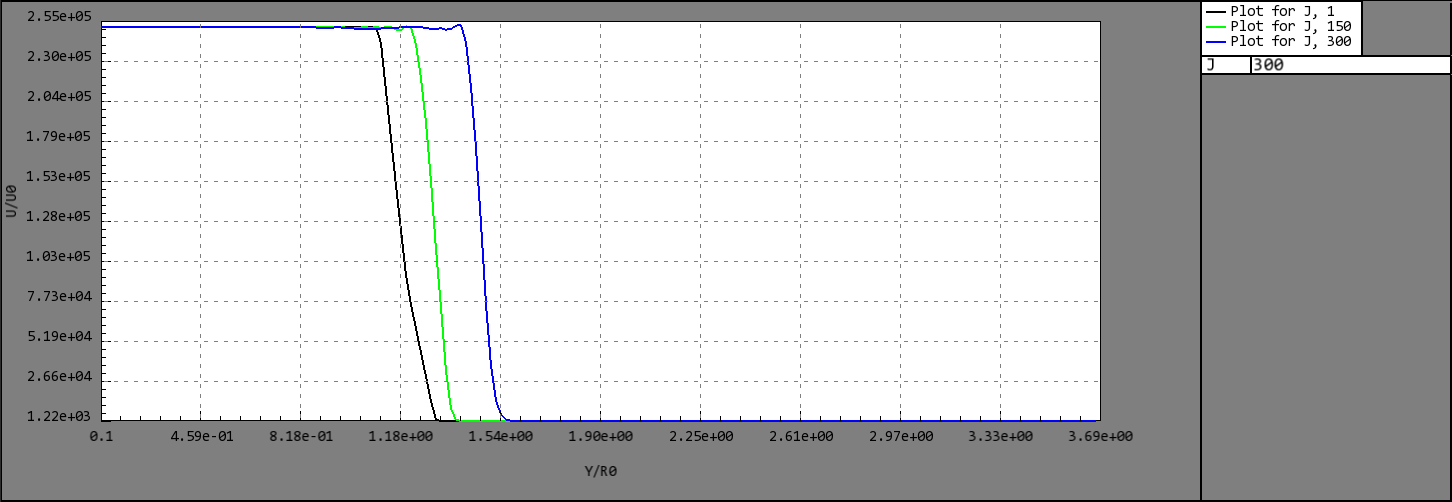
\includegraphics[width=15cm]{2-05-test-J}
    \caption{Значения энтальпии $J$}
    \label{fig:acc_J}
\end{figure}

\begin{figure}
    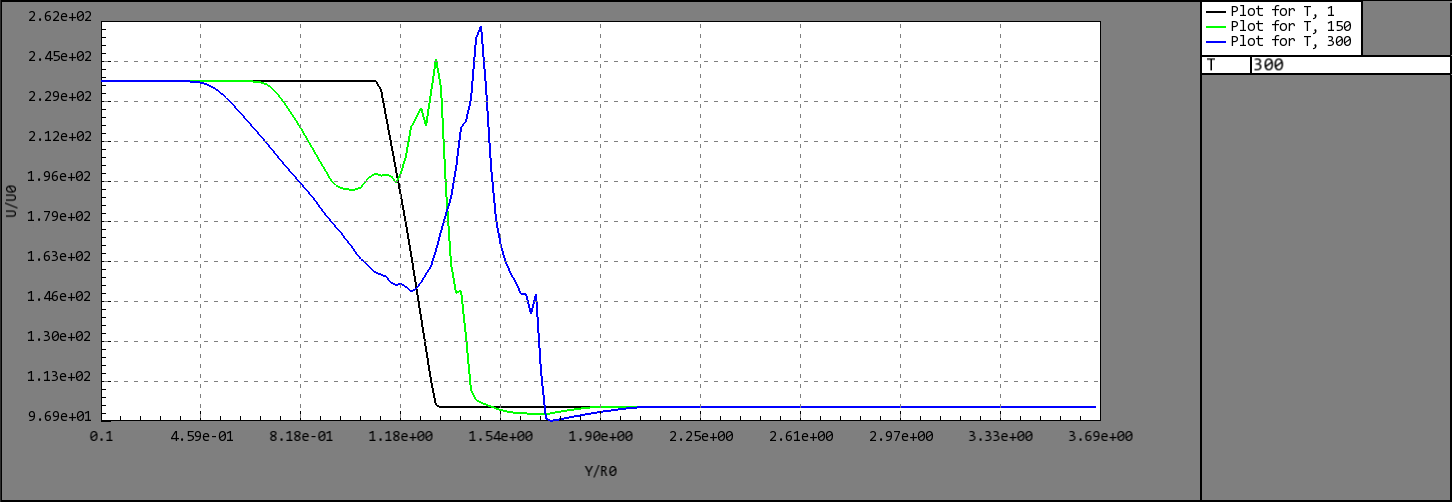
\includegraphics[width=15cm]{2-05-test-T}
    \caption{Значения температуры $T$}
    \label{fig:acc_T}
\end{figure}

\begin{figure}
    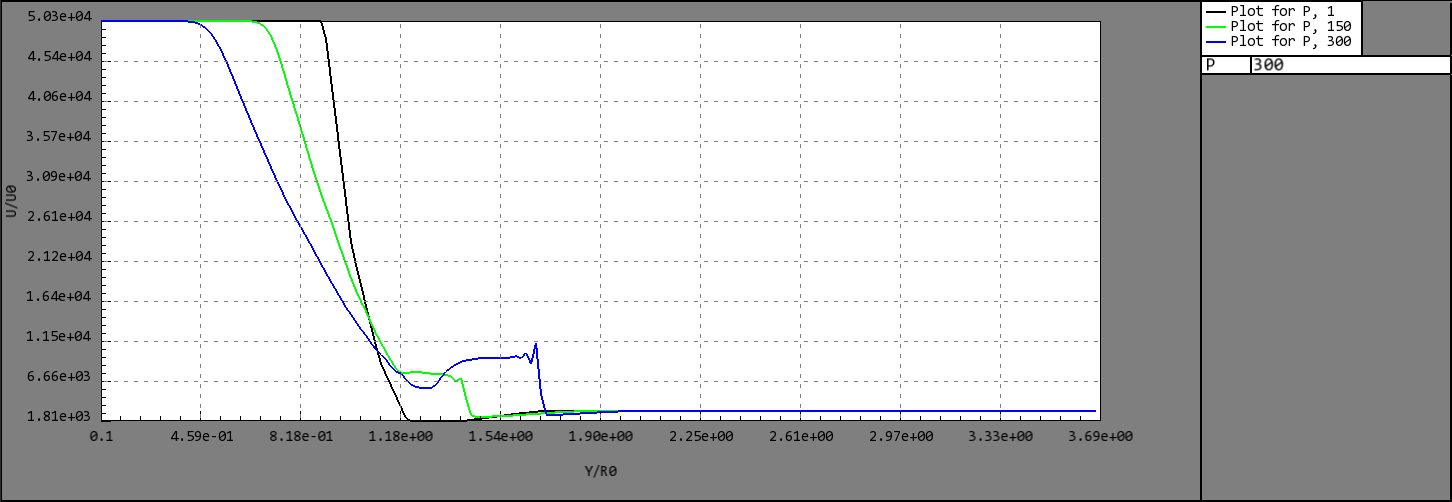
\includegraphics[width=15cm]{2-05-test-P}
    \caption{Значения давления $P$}
    \label{fig:acc_P}
\end{figure}

\begin{figure}
    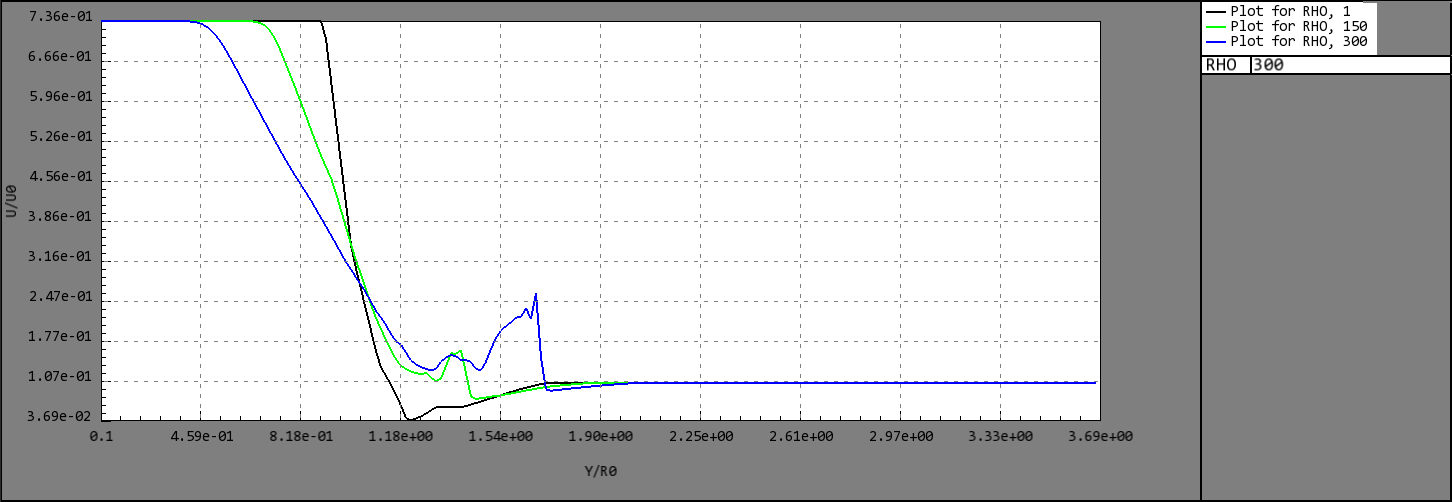
\includegraphics[width=15cm]{2-05-test-RHO}
    \caption{Значения плотности $\rho$}
    \label{fig:acc_RHO}
\end{figure}

Проведенные тесты показали:
\begin{itemize}
\item Параболизированная постановка обеспечивает разумный компромисс между точностью и производительностью
\item Оптимальный шаг дискретизации составляет $\Delta x \approx 0.03L$
\item Время расчёта растет почти квадратично с увеличением числа узлов (уменьшением шага)
\end{itemize}
    
    \conclusion

Проделанная работа представляет собой программу для работы с СДУ при помощи множества методов семейства Рунге-Кутты. В работе
реализовано 18 явных методов со 2 по 6 порядок точности, 9 вложенных, включая схему Дормана-Принца 4-5 порядка, 22 неявных, в том числе
схемы Радо, Гаусса и Лобатто для полных и неполных матриц. Помимо этого, протестирован один L-стабильный диагональный метод. Для
неявных схем используются схемы решения СЛАУ первого порядка (простой итерации, Зейделя) и второго порядка (метод Ньютона), причём
для обращения
матрицы применялся метод LU-разложения. Для дифференцирования функции при построении матрицы Якоби для метода Ньютоны использовались
формулы с 4 порядком точности. При необходимости можно использовать формулы с меньшим порядком.

Для того чтобы определить, какие методы можно использовать, был реализован алгоритм вычисления числа жёсткости СДУ, использующий
QR-разложение матрицы системы для поиска всех собственных чисел. При высокой жёсткости для расчёта применяютя только жёсткие
схемы.

Для удобного отображения результатов вычислений был создан генератор pdf-отчётов, в которых представлена информация о решаемой задаче,
метод её решения и таблица Бутчера для этого метода, график, отображающий решение численными методами и аналитическое (при наличии) и
время, затраченное на работу программы. Если задача решалась при помощи жёстких схем, то дополнительно выводится информация о
количестве итераций. Так же, при необходимости, может быть построен приближающий полином. Кроме этого, реализована возможность простого
добавления новых методов решения на случай, если пользователю нужно решение каким-либо специфическим методом, которого нет в программе.
При помощи пользовательского интерфейса можно использовать разработанную программу как для решения ОДУ, так и в целях обучения.

Программа тестировалась как на задачах химической кинетики, так и на модельных уравнениях и дала удовлетворительные результаты. % Заключение

    \printbibliography % Список литературы

    \appendix % Приложения
    \appendixsection{Исходный код}
    
Исходный код программы выложен в публичном репозитории GitHub. QR код на репозиторий представлен на рисунке \ref{fig:a1}.

\begin{figure}
    
\includegraphics[width=5cm]{qr_code}
    \caption{Рисунок в приложении}
    \label{fig:a1}
\end{figure}
    %\appendixsection{Приложение с таблицей}

Таблица~\ref{tab:b1} идёт с нумерацией приложения.

\begin{table}    
    \caption{Пример короткой таблицы с использованием tabular}
    \begin{tabular}{|r|c|c|c|l|}\hline
    Тело      & $F$ & $V$  & $E$ & $F+V-E-2$ \\ \hline
    Тетраэдр  & 4   & 4    & 6   & 0         \\ \hhline{~-~-~}
    Куб       & 6   & 8    & 12  & 0         \\ \hhline{--~~~}
    Октаэдр   & 8   & 6    & 12  & 0         \\ \hhline{-----}
    Додекаэдр & 20  & 12   & 30  & 0         \\ \hline
    Икосаэдр  & 12  & 20   & 30  & 0         \\ \hline
    \end{tabular}
    \label{tab:b1}
\end{table}

\lipsum[1][1]

    %\appendixsection{Приложение с формулой}

Формула~\ref{c1} также идёт с нумерацией приложения.

\begin{equation}
    2 + 2 = 4
    \label{c1}
\end{equation}

    %\appendixsection{Приложение с листингом}

Рисунок~\ref{src:src3} с листингом в приложении.

\begin{figure}
\lstinputlisting[language=C++]{inc/example.cpp}
\caption{Пример использования листинга}
\label{src:src3}
\end{figure}
\end{document}
